%=========================================================================

\chapter{Introduction}
This chapter describes the motivation leading to the presentation of this paper and how is it related to the SLAM++ project at FIT VUT. The objectives of the project and the subjects included in this document are briefly explained. The chapter ends describing the overall structure and contents of the remaining of the paper.

\section{Motivation}
There is an immerse need to record and preserve our knowledge and perception of the world around us. Evidence of such tendency can be track thousands of years back in human existence as a cave paintings. Later we used more advanced techniques in form of written languages, sculptures, drawings, et cetera. Nowadays we have means to record our surroundings as we perceive it in 2D using cameras. However, it has proven difficult to process such information digitally. Even automated analysis of 2D information like typeset books is not a trivial problem and far from being mastered. While there are so called OCR converters available, in many cases they don't work reliably enough.

When it comes to 3D the problem gets much more difficult. Scanning 3D object reliably is nowadays possible in laboratory conditions, but there are hard limits like the size of the object, its structure or surface and material properties. Also the laboratory equipment used is much more expensive and physically larger compared to its 2D counterpart. This paper tries to address both of these problems by allowing user to create 3D model using multiple pictures of an object of interest from various sources. Such 3D model, even though it may be inaccurate, has number of applications. It can be used by archaeologists to preserve cultural heritage, by architects for spatial planning, by entertainers to create 3D models and virtual reality or by engineers to replicate existing 3D objects.

\section{Tools}
The process of creating a 3D model usually consist of two parts: scanning the object and reconstruction of the model. There are three main approaches how to scan physical object: contact, active non-contact  and passive non-contact scanners. The contact 3D scanners probe the subject through physical touch. The active non-contact scanners use a light in forms of laser or X-ray to scan the object while the passive non-contact scanners are using either multiple cameras, images with varying lighting conditions or silhouettes extruded from image with contrasted background. In this thesis we will be particularly interested in scanning objects using multiple images from various cameras. We will talk more about this in next chapter \ref{chapter:methodology} but for now note that for this we will use the SLAM++ framework \cite{www:slam}. The output of such scanning is usually a set of 3D points with a color information called point cloud. These data have to be filtered in order to remove noise, segmented and then reconstructed into polygonal model. The reconstruction can be done either manually using software like MeshLab \cite{www:meshlab} or automatized with framework like the PCL \cite{www:pcl}. 

\section{Objectives}
This paper aims to identify challenges of 3D reconstruction from a set of 2D images taken by various cameras leading to creation of a software that can do so automatically. The objective deals with the aim of reducing the correspondence problem between each two images and the study of camera modelling and calibration. An accurate estimation of the camera model and correspondence allows us to compute three-dimensional information from a two-dimensional image sequence. In order to eliminate artefacts the input set of images, obtained from internet, will have to be filtered to contain only daytime images from summer season.

The study of the geometry involved in multiple camera vision systems should allow us to present an application that can from a set of two-dimensional images reconstruct 3D scene depicted by the images.

\section{Overall Structure}
This paper consist of 4 chapters and a bibliography at the end of the document.

Chapter \ref{chapter:the-state-of-the-art} introduces reader to the process of estimation three-dimensional structure from two-dimensional image sequences. Firstly, it discuss existing solutions, like VisualSFM, photosynth and Bundler, elaborated on the output of these programs. Later they will be used as a benchmark for the implemented application. These will be used for the final application performance and effectiveness evaluation.. Then it focuses on the state-of-the-art features detectors, extractors and matchers, built in the SLAM++ frontend, and aims to compare theirs efficiency and performance. The comparison is then discussed and best combination in terms of performance and effectiveness chosen for the planned application.

In the chapter \ref{chapter:methodology} the whole 3D reconstruction process is thoroughly discussed and step by step explained. The steps that are already implemented, like dataset acquisition or feature detection, extraction and matching, are in detail described. The rest of the pipeline is also outlined to give the reader idea what are the next steps to be implemented. 

Finally, chapter \ref{chapter:conclusion} summarizes this document by discussing achieved goals.

\chapter{The State of the Art}
\label{chapter:the-state-of-the-art}
The following chapter presents to the reader the process of estimating three-dimensional structures from two-dimensional image sequences. After brief introduction into the pipeline, some of the existing solutions for the Structure from Motion (SfM) imaging technique are discussed. The programs described will be used as a benchmark for the final solution once it's presented. We take a closer look on first part of the pipeline consisting of the feature detectors, extractors and matchers. The goal is to select the best combination in terms of performance and effectiveness for reconstruction of historic landmarks. 

\section{Existing 3D Reconstruction Solutions}
The problem of creating 3D reconstruction from set of images has been addressed by many research groups. In this section we will talk about few of the widely known solutions. All of the programs below implement a subset of algorithm for structure from motion which consist of 7 distinct steps:
\begin{itemize}
	\item[1)] \textbf{Dataset aquisition.} First step in the SfM pipeline is selection of a input data. Specific requirements on the data varies throughout different software, however, we can generalize some properties of such set of images. The set has to contain images that are overlapping one another. Only such images are used in the reconstruction as they provide points seen by multiple cameras and therefore the 3D position can be calculated.
	\item[2)] \textbf{Keypoints detection.} Keypoints are parts of the image that are significant in some way. The significance is usually caused by a sudden change in gradient on relatively small part of the image. These points will be used to estimate the 3D representation. We will focus more on keypoints detection in section \ref{sec:detectors}. 
	\item[3)] \textbf{Feature extraction.} The detected keypoints are rarely used as provided by the detector as they do not provide enough information about the point itself. A set of calculations is applied in order to extract data from the surroundings of such point and enrich information about the keypoint. Resulting structure is called feature and contains all data required for next step. At this point the input image does not have to be kept in memory anymore.
	\item[4)] \textbf{Feature matching.} Now that we have keypoints represented as feature we want to establish a visual correspondence between a set of keypoints from two closely related images. This is done by so called feature matching and will be discussed in detail in section \ref{sec:matchers}.
	\item[5)] \textbf{Camera initialization and pose estimation.} Once we know correspondence between two closely related images, we can estimate the parameters of the camera(s). If not known, the camera matrix can be calculated and the relation between the points in 3D.
	\item[6)] \textbf{Structure computation.} Next step is to calculate the model's 3D structure from the points seen by different cameras. The quality of the structure is greatly affected by errors from previous steps.
	\item[7)] \textbf{Visualization.} Lastly the resulting 3D structure in form of point cloud is visualized.The visualization can be either just a set of images cleverly arranged to give impression of 3D, cloud of 3D points or polygonal model. In this thesis we will not be interested in the visualization of the resulting model, however we see this as an important part of the SfM pipeline.
\end{itemize}

\subsection*{Photosynth}
Photosynth is a software application developed by Microsoft. It is based on Photo Tourism, a research project by University of Washington graduate student Noah Snavely. Formerly the Photosynth was a 3D reconstruction software, however, in the current version output of the application is not a point cloud nor 3D model but an animation of morphing images or panorama. While it still works with images from various sources, the best result is achieved by importing photos from a single camera. Once imported, user has to choose the camera trajectory from four predefined options: spin, panorama, wall or walk. 

The Photosynth technology is using an interest point detection and matching algorithm developed by Microsoft Research which is similar in function to SIFT. Detected features are then matched between images and by analyzing subtle differences in the relationships between the features (angle, distance, etc.), the program identifies the 3D position of each feature, as well as the position and angle at which each photograph was taken. Everything is processed by Microsoft's servers and, once finished, pushed to the website or desktop/mobile application. There are little to none information about the whole process as this is a commercialized technology. \cite{www:photosynth}

\begin{figure}[ht]
	\begin{center}
		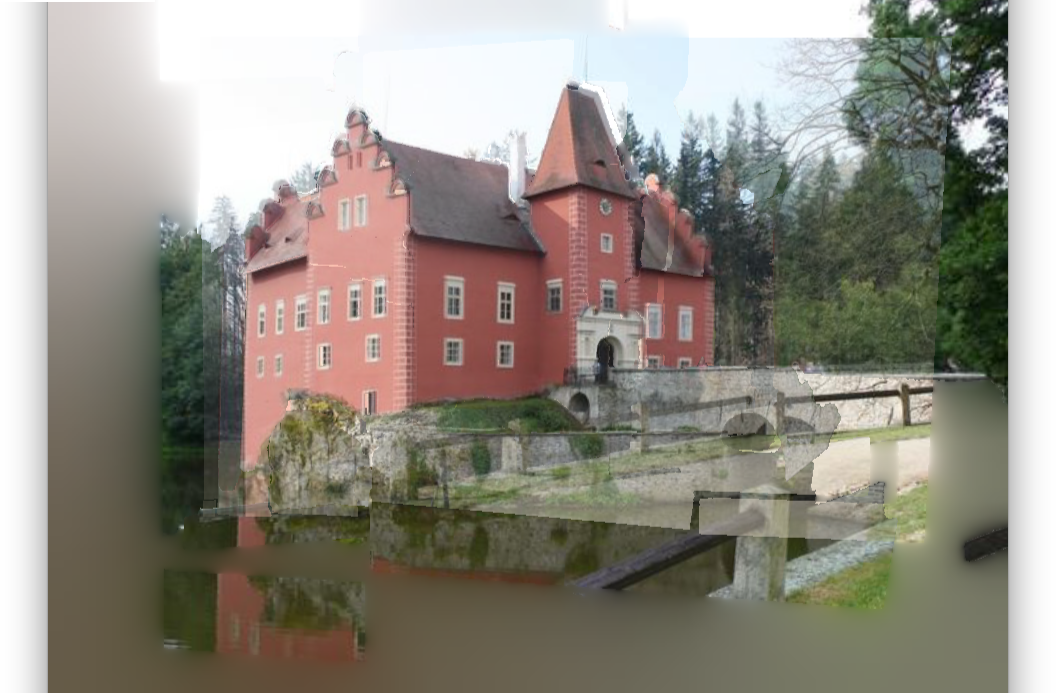
\includegraphics[keepaspectratio,width=\textwidth]{fig/Photosynth.png}
	\end{center}
	\caption{The Photosynth output of the Červená Lhota Castle in transition between several morphed images.}
	\label{fig:visualsfm}
\end{figure}

\subsection*{VisualSFM}
The Chungchang Wu's Visual Structure from Motion System is a GUI application for 3D reconstruction using structure from motion (SFM). The reconstruction system is modular and integrates several of other projects: SIFT on GPU(SiftGPU), Multicore Bundle Adjustment, and Towards Linear-time Incremental Structure from Motion. VisualSFM runs fast by exploiting multicore parallelism for feature detection, feature matching, and bundle adjustment. For dense reconstruction, the program supports Yasutaka Furukawa's PMVS/CMVS tool chain, and can prepare data for Michal Jancosek's CMP-MVS. In addition, the output of VisualSFM is natively supported by Mathias Rothermel and Konrad Wenzel's SURE.

The software follows the overall 3D reconstruction pipeline; It detects features using SIFT detector and SIFT extractor, matches feature pairs with the N-View Match, estimates the camera model for each image, removes images' distortion and then runs the dense reconstruction. Outputs of feature extraction and matching are stored as a binary files and are loaded if provided to save processing time. This enables use of other than built-in extractors and matcher, at least for the sparse reconstruction. \cite{www:visual_sfm}

\begin{figure}[ht]
	\begin{center}
		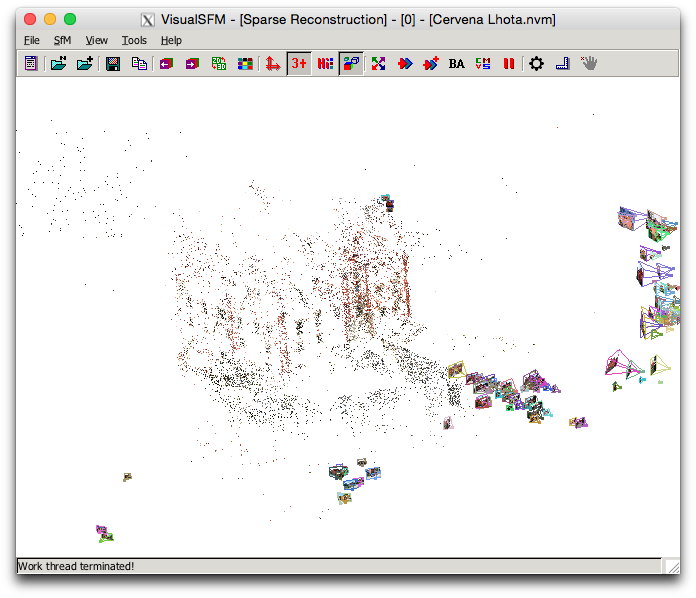
\includegraphics[keepaspectratio,width=\textwidth]{fig/VisualSFM.png}
	\end{center}
	\caption{The VisualSFM application GUI with sparse reconstruction of the Červená Lhota Castle.}
	\label{fig:visualsfm}
\end{figure}

\subsection*{Bundler}
Bundler is first well known Structure from Motion (SfM) system for unordered image collections from Noah Snavely. One of the first version of this Bundler system was used in the Photo Tourism project that was aqired by Microsoft and is now part of Photosynth. 

As other applications discussed, Bundler takes a set of images, image features, and image matches as input, and produces a 3D reconstruction of camera and sparse scene geometry as output. In order to get sparse point clouds, one has to run Bundler to get camera parameters, use the Bundle2PMVS program to convert the results into PMVS2 input and then run PMVS2. The system reconstructs the scene incrementally, a few images at a time, using a modified version of the Sparse Bundle Adjustment package of Lourakis and Argyros as the underlying optimization engine. Bundler has been successfully run on many Internet photo collections, as well as more structured collections. \cite{www:bundler}

\section{Detectors}
\label{sec:detectors}
A successful 3D reconstruction stands and falls on good features detection.The quality and robustness of features is (usually) much more important then their quantity which will be demonstrated by the Dense detector later in this section. The ideal feature detector finds salient image regions such that they are repeatedly detected despite change of viewpoint; more generally it is robust to all possible image transformations. Therefore, it does not detect any points in uniform and uninteresting surfaces like sky or texture-less walls. The best detector to be used depends heavily on the requested task. In our application features we are interested in are edges and corners of buildings and their distinct parts.

We can divide types of image features into following categories (please note that a detector can detect features from multiple categories):
% CITATION NEEDED!!!
\begin{itemize}
	\item \textbf{Edge} is a point where there is a sudden change between adjacent pixels (strong gradient magnitude). Generally an edge can be of almost any arbitrary shape and may include junctions. Locally edges have a one-dimensional structure.
	\item \textbf{Interest point} has a local two dimensional structure. We can think of it as two-dimensional edge, in fact early algorithms were used to detect interest points as edges and then selected the interest points by further calculation. In some literature you the interest points may be referred to as corners.
	\item \textbf{Blobs} provide a complementary description of image structures in terms of regions, as opposed to corners that are more point-like. A term regions of interest or interest points are sometimes used as the blob descriptors often contain a preferred point (a local maximum or a center of gravity). Blobs allows detection of smooth areas in an image that might not be detected as an edge or corner.
	\item \textbf{Ridges} are in computer vision a set of curves whose points are have a local maximum in at least one dimension. This notion captures the intuition of geographical ridges. Ridge detection is usually much harder then Edge, Interest point or Blob detection.
\end{itemize}

In the remainder of this section feature detectors implemented in the SLAM++ frontend using OpenCV will be presented. Each detector will be run on the same set of images with historic landmarks in order to evaluate the effectiveness and speed. Then a summary of the results will be presented.
 
\begin{itemize}
	\item The \textbf{Robust Invariant Scalable Keypoints (BRISK)} detector uses scale-space pyramid layers of octaves and intra-octaves to detect corners in an image. The algorithm uses FAST feature detector score and was developed to get the better of SIFT and SURF detectors. However, in our case the performance gain is not worth decreased feature quality. \cite{article:brisk}
	
	\item \textbf{Dense Sampling} uses a regular grid to find a keypoints in the image. This results in good coverage of the entire object or scene and a constant amount of feature per image area. The dense sampling is fast as the detector selects all points on a grid without analysis of the surrounding. On the downside, dense sampling cannot reach the same level of repeatability as obtained with interest points, unless sampling is performed extremely densely, but then the number of features quickly grows unacceptably large. The dense sampling is therefore not useful in the SfM model estimation, but can be used for a dense reconstruction once sparse structure is calculated. \cite{article:dense}
	
	\item The \textbf{Features from Accelerated Segment Test (FAST)} aims to rapidly increase performance of feature detection while sustaining feature quality of SIFT-like detectors. The algorithm detects corners in the image and should be used with SIFT or SURF extractor for best performance. As the FAST select in our case three times more features hundred times faster than SIFT (resp. 50 times faster than SURF) we market this as one of the interesting detectors for the final implementation. \cite{article:fast}
	
	\item One of the most known feature detectors is the \textbf{Harris Corner Detector} . It can identify similar regions between images that are related through affine transformations and have different illuminations. Even though the Harris Corner Detector is fast, it does not select enough keypoints and therefore is not suitable for the 3D building reconstruction. \cite{www:harris}
	
	\item The \textbf{Good Features to Track (GFTT)} detector is modified version of the Harris Corner Detector described earlier. It is still classified as a corner detector, however, the scoring function differs. Compared to the Harris, the algorithm was slightly slower, with higher amount of features. Nevertheless, both of these algorithms do not perform well enough for our problem. \cite{article:gftt}
	
	\item The \textbf{Oriented FAST and Rotated BRIEF (ORB)} detector originated from the OpenCV Labs. It's goal was to offer robustness of a SIFT and SURF, while maintaining fast processing time like FAST and BRIEF combination. While this may be true, for our problem the ORB detector does not perform well enough. The feature found rarely belong to a building and usually chunks around trees and vegetation. \cite{www:orb}\cite{article:orb}
	
	\item The \textbf{Maximally Stable Extremal Regions} is a blob detector. For our task this detector performs poorly and takes even more time than SIFT detector.
	
	\item A \textbf{Scale Invariant Feature Transform (SIFT)} keypoint is image region with an orientation. The detector uses as a keypoints image structures  which resemble blobs. The use of the detector is licenced which is one of the reasons why we would like to use a different detecter. However, as expected, the detector performs very well and is used by other SfM software we discussed earlier. \cite{article:sift}
	
	\item The \textbf{Speeded Up Robust Features} detector is modification of the SIFT detector. It addresses slow processing of the SIFT while maintaining reasonable efficiency. While it can surely be used in the SfM application, from our experiments we discovered that the increased performance greatly decreases feature detection for (in our case) important structures.  \cite{www:surf}
\end{itemize}

We've implemented all of the standard OpenCV keypoints detectors from previous list in the SLAM++ frontend. The goal was to test how do they perform on our specific problem: detecting keypoints in buildings. The figure \ref{fig:detectors} shows three detectors (SIFT, SURF and FAST) that are suitable for our task as they find enough relevant features in an image. 

\begin{figure}[ht]
	\begin{center}
		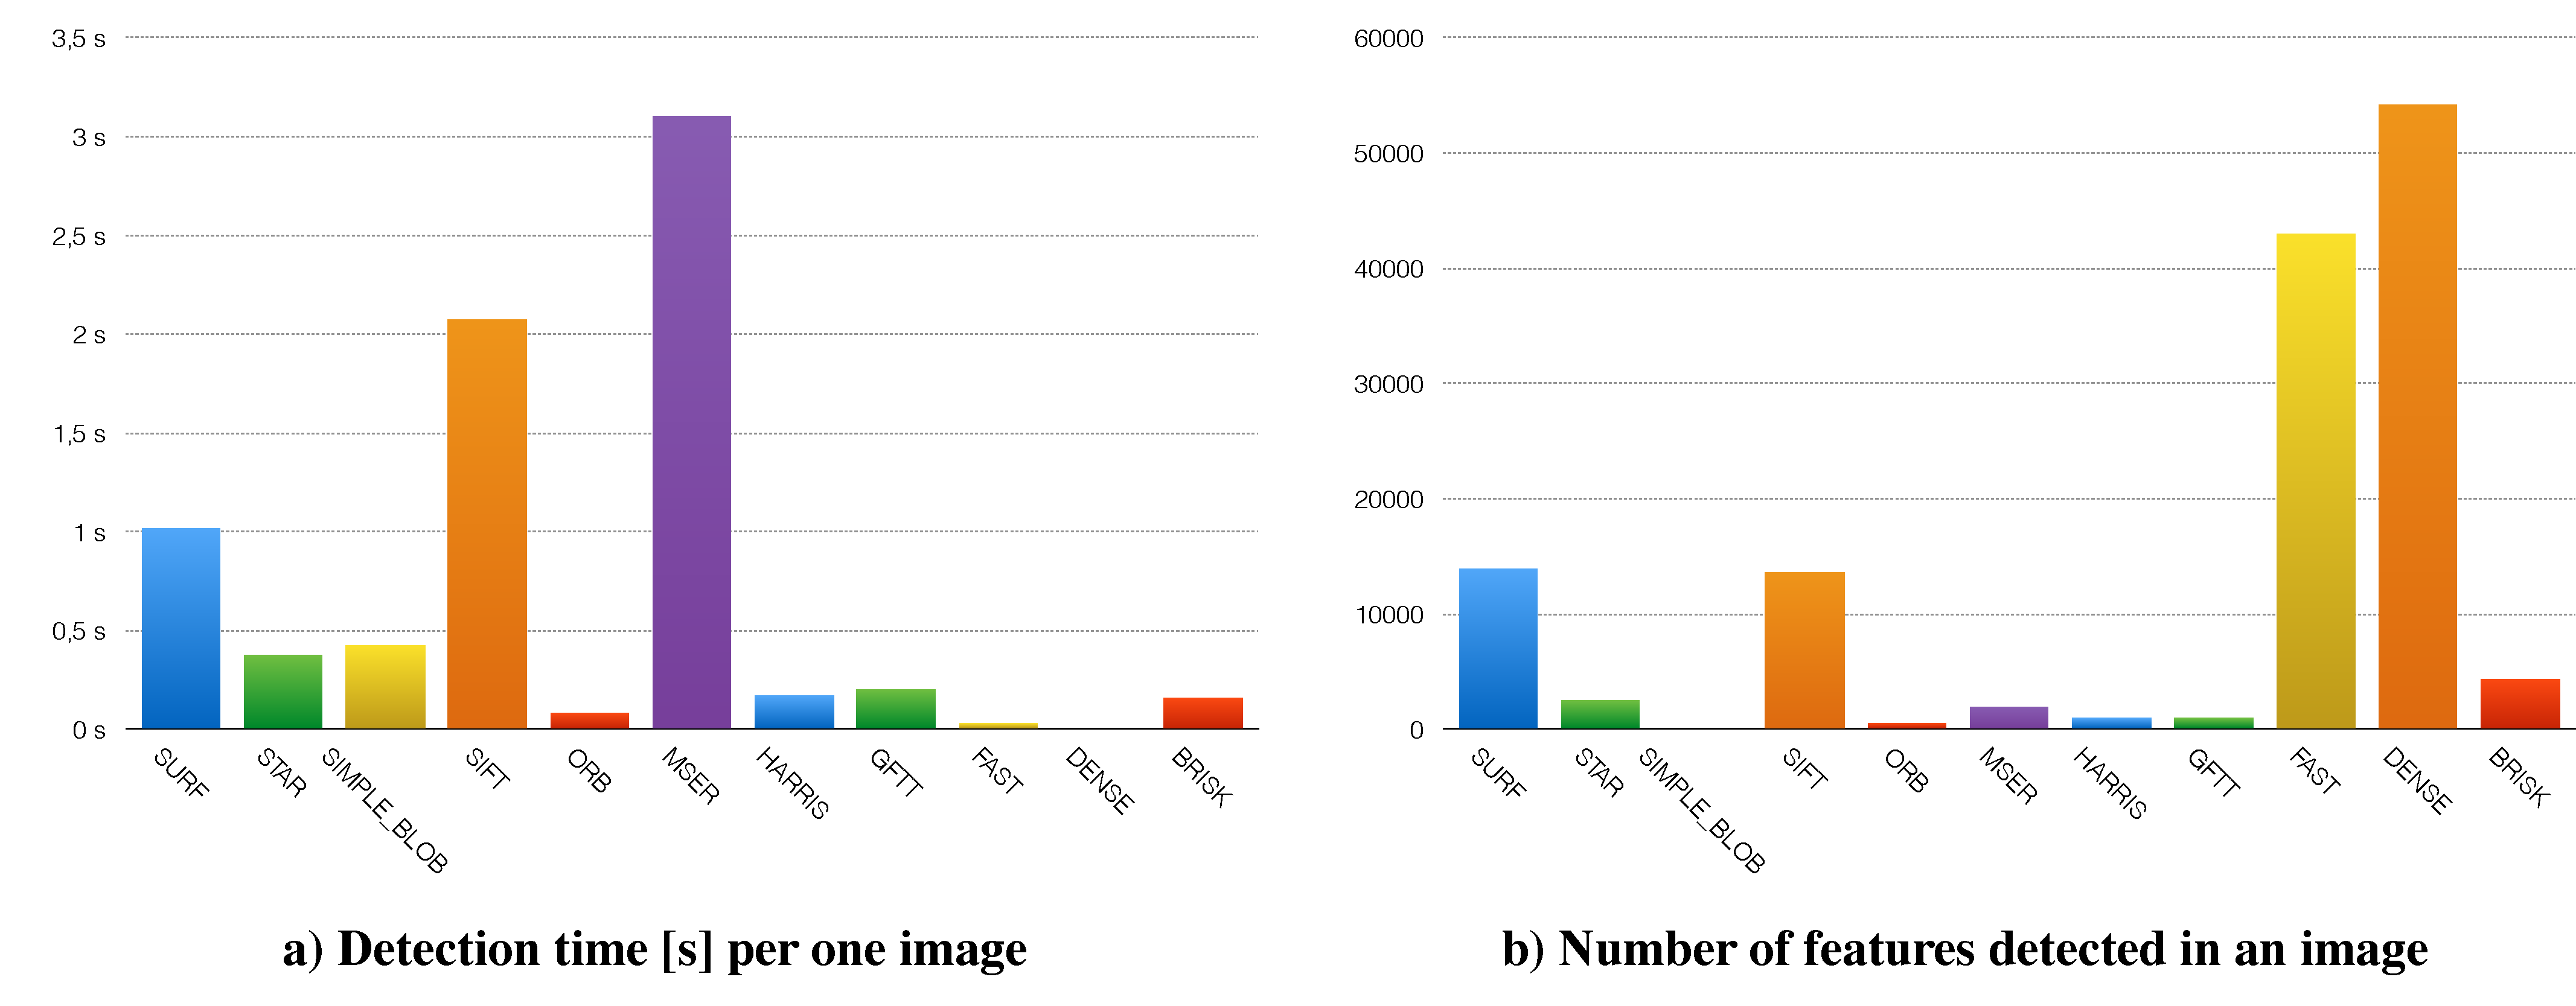
\includegraphics[keepaspectratio,width=\textwidth]{fig/detectors.pdf}
	\end{center}
	\caption{Results of the feature detection evaluation on as set of 500 various images from the Červená Lhota dataset. Graph a) shows average time necessary for processing an image using selected detector. In graph b) you can find how many features on average were detected in a single image.}
	\label{fig:detectors}
\end{figure}

\section{Extractors}
\label{sec:extractors}
Once features have been detected, a local image patch around the feature can be extracted. This extraction may involve quite considerable amounts of image processing. The result is known as a feature descriptor or feature vector. Among the approaches that are used to feature description, one can mention N-jets and local histograms. In addition to such attribute information, the feature detection step by itself may also provide complementary attributes, such as the edge orientation and gradient magnitude in edge detection and the polarity and the strength of the blob in blob detection.

\begin{itemize}
	\item \textbf{SIFT:} The scale-invariant feature transform of a neighbourhood is a 128-dimensional vector of histograms of image gradients. The region, at the appropriate scale and orientation, is divided into a $4\times 4$ square grid, each cell of which yields a histogram with 8 orientation bins.
\end{itemize}
\section{Matchers}
\label{sec:matchers}

\section{Feature Based Image Registration}

\chapter{Methodology}
\label{chapter:methodology}
This chapter describes the process of 3D reconstruction from a set of images to the point cloud output. It puts the features detection, extraction and matching into context of 3D reconstruction. In order to select only inliers, the RUNSAC algorithmes filters the matched feature pairs. Then, using mathematical apparatus from chapter \ref{chapter:theoretical-background} the fundamental matrix and camera model are estimated. Finally, once we know the camera model, we can run dense reconstruction, creating the resulting point cloud.  
\section{Three-dimensional Structure Estimation Pipeline}
\subsection*{Selecting Dataset}
\subsection*{Feature Detection and Extraction}
\subsection*{Feature Matching}
\section{3D Reconstruction Approaches}
Stereo, Mono, Uncalibrated
frontend and backend

\chapter{Conclusion}
\label{chapter:conclusion}

%=========================================================================
